\documentclass{beamer}
\usepackage{tcolorbox}
\usepackage{hyperref}
\usepackage{../notation}
\usepackage{subfig}

%\beamerdefaultoverlayspecification{<+->}
% \newcommand{\data}{\mathcal{D}}
% \newcommand\Item[1][]{%
% 	\ifx\relax#1\relax  \item \else \item[#1] \fi
% 	\abovedisplayskip=0pt\abovedisplayshortskip=0pt~\vspace*{-\baselineskip}}

\graphicspath{ {imgs/} }

\usetheme{metropolis}           % Use metropolis theme


\title{Bias-Variance}
\date{\today}
\author{Nipun Batra and teaching staff}
\institute{IIT Gandhinagar}
\begin{document}
	\maketitle

\begin{frame}{The Scenario: True Function}
\vspace*{0.4cm}
For the purpose of this lecture we assume that there exists a relation between \textbf{Housing Prices} and \textbf{area of the house}.
\pause

Here, the true function $f_{\theta (true)}$ is used to model the relation $y_i = f_{\theta (true)}(x_i)$
\begin{figure}
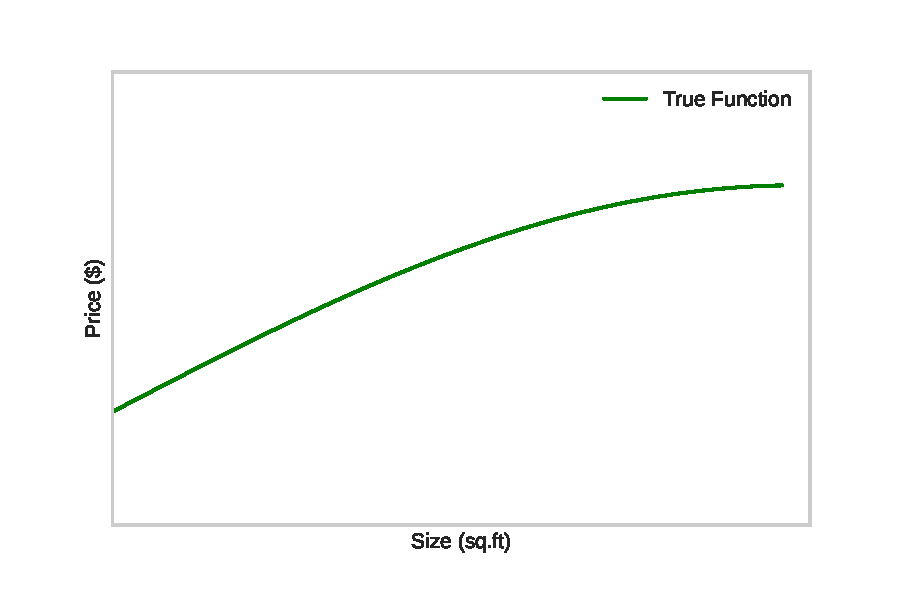
\includegraphics[width=0.7\textwidth]{images/true.pdf}
\vspace*{-0.3cm}
\caption{Modeling the relation}
\end{figure}
\end{frame}

\begin{frame}{The 3 Sources of Error}
Any prediction made is effected by 3 sources of error:
\begin{itemize}
\item Noise
\item Bias
\item Variance
\end{itemize}
\end{frame}

\begin{frame}{Noise}
\vspace*{0.4cm}

\only<1-2>{Data is inherently noisy. This stems from the fact that no relation can model all possible attributes. }

\only<2-2>{So a relation between \textbf{price} and \textbf{size} will be affected by other factors such as the \textbf{condition of the house}.}
\only<3->{This is \textbf{not} a property of data and is an \textbf{Irreducible error}. 
It can be understood by the equation: $y_i = f_{\theta (true)}(x_i)+\epsilon_i$
}

\only<4->{The noise is mean centered around the true function and has spread that is called the variance of the noise}
\vspace*{-0.6cm}
\only<2-3>{\begin{figure}
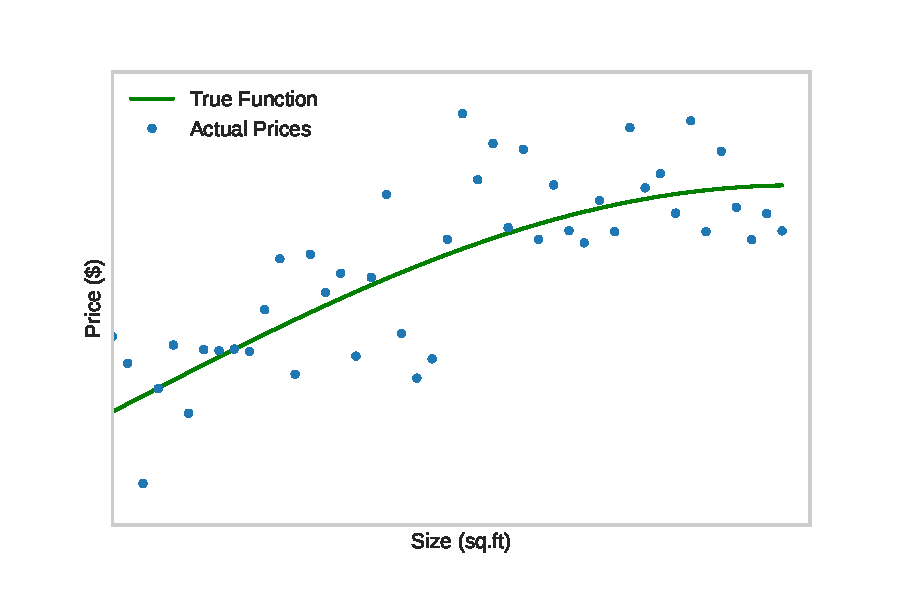
\includegraphics[width=0.7\textwidth]{images/data.pdf}
\vspace*{-0.3cm}
\caption{Modeling the relation}
\end{figure}}
\only<4->{\begin{figure}
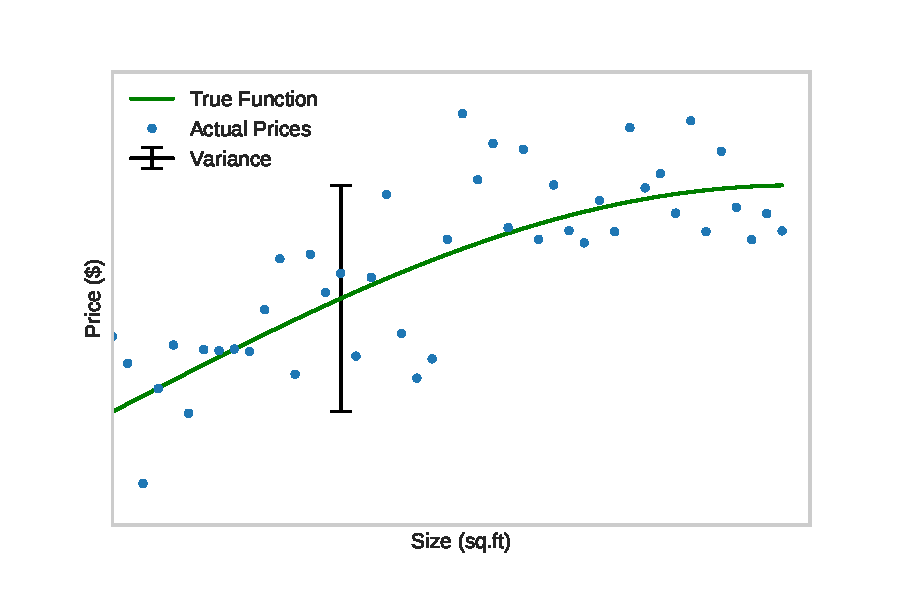
\includegraphics[width=0.7\textwidth]{images/data_var.pdf}
\vspace*{-0.3cm}
\caption{Modeling the relation}
\end{figure}}

\end{frame}

\begin{frame}{Bias}
\vspace*{0.4cm}
\only<1-4>{\textbf{Bias} is a measure of how well can the model fit the true relation between the parameters.}

\only<2>{Assume that we have two datasets of houses sold.}
\only<2>{\begin{figure}
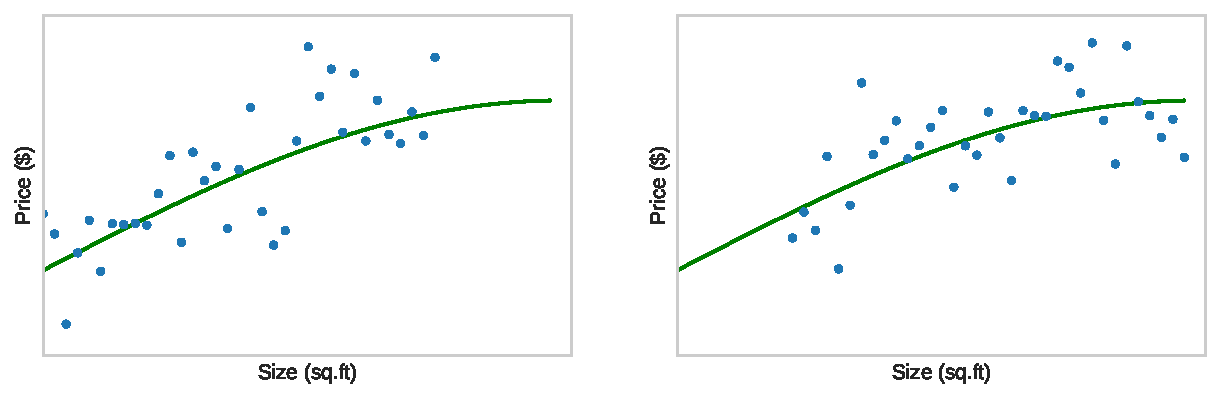
\includegraphics[width=\textwidth]{images/bias1.pdf}
\vspace*{-0.3cm}
\caption{Two Datasets from same relation}
\end{figure}}

\only<3>{If we try to fit a constant function to them.}
\only<3>{\begin{figure}
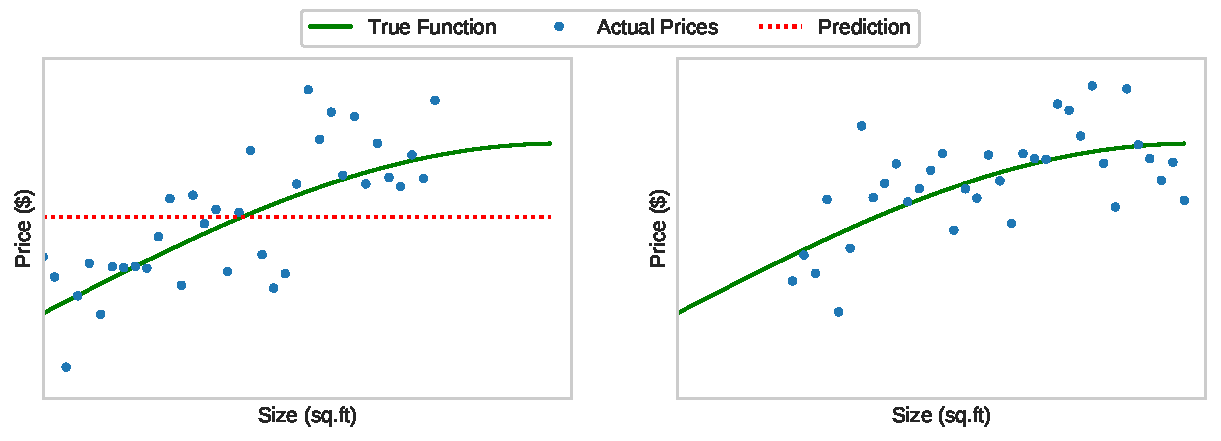
\includegraphics[width=\textwidth]{images/bias2.pdf}
\vspace*{-0.3cm}
\caption{Two Datasets from same relation}
\end{figure}}

\only<4>{We see that they show different predictions.}
\only<4>{\begin{figure}
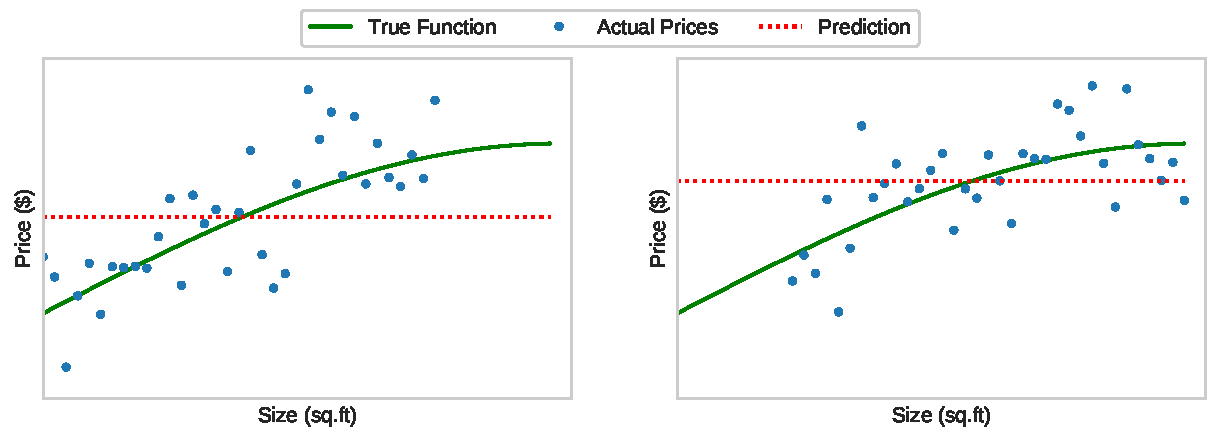
\includegraphics[width=\textwidth]{images/bias3.pdf}
\vspace*{-0.3cm}
\caption{Two Datasets from same relation}
\end{figure}}

\only<5>{Doing so for all possible size N training sets we get}
\only<5>{\begin{figure}
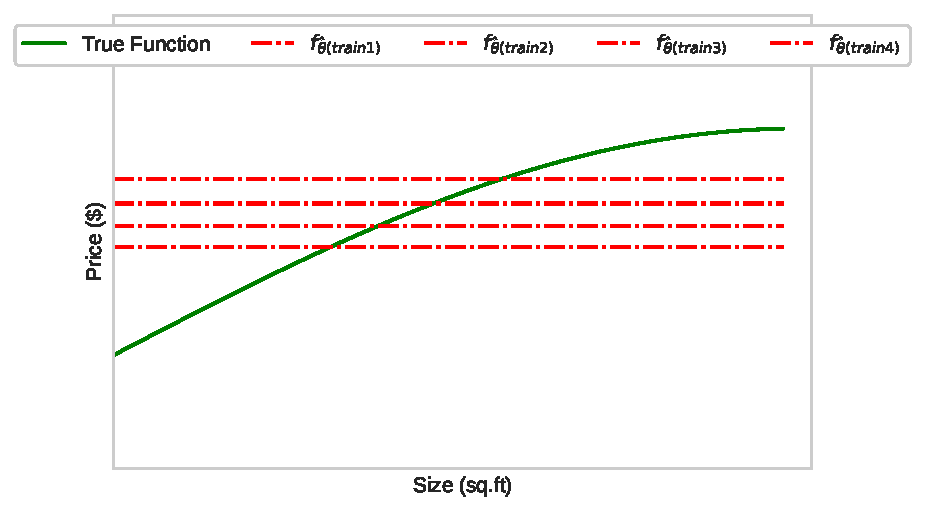
\includegraphics[width=\textwidth]{images/bias4.pdf}
\vspace*{-0.6cm}
\caption{Fits on different training sets}
\end{figure}}

\only<6>{Averaging all the fits (based on their likelihood) we get the average fit.}
\only<6>{\begin{figure}
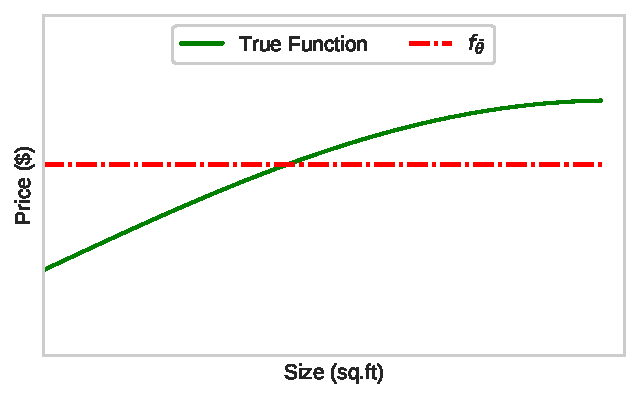
\includegraphics[width=0.7\textwidth]{images/bias5.pdf}
\vspace*{-0.3cm}
\caption{Average fit on all different training sets}
\end{figure}}

\end{frame}

\begin{frame}{Bias Contribution}
\only<1->{$$\text{Bias}(x) = f_{\theta(true)}(x) - f_{\bar\theta}(x)$$}
\only<2->{It is measure of how flexible the fit is in capturing $f_{\theta(true)}(x)$}
\only<1->{\begin{figure}
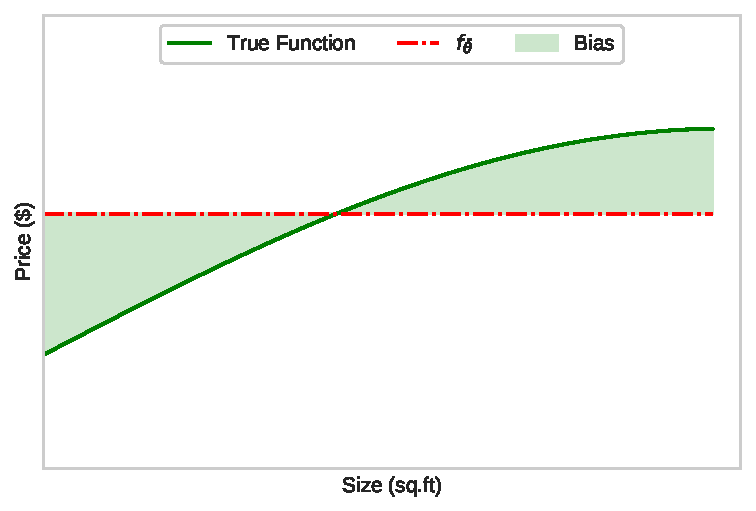
\includegraphics[width=0.7\textwidth]{images/bias6.pdf}
\vspace*{-0.3cm}
\caption{Bias of the fit}
\end{figure}}

\end{frame}

\begin{frame}{Bias Contribution: Effect of Complexity}
\only<1>{As we increase the complexity of the fit \\ $\implies$ fit becomes more flexible \\ $\implies$ bias decreases}
\only<1>{\begin{figure}
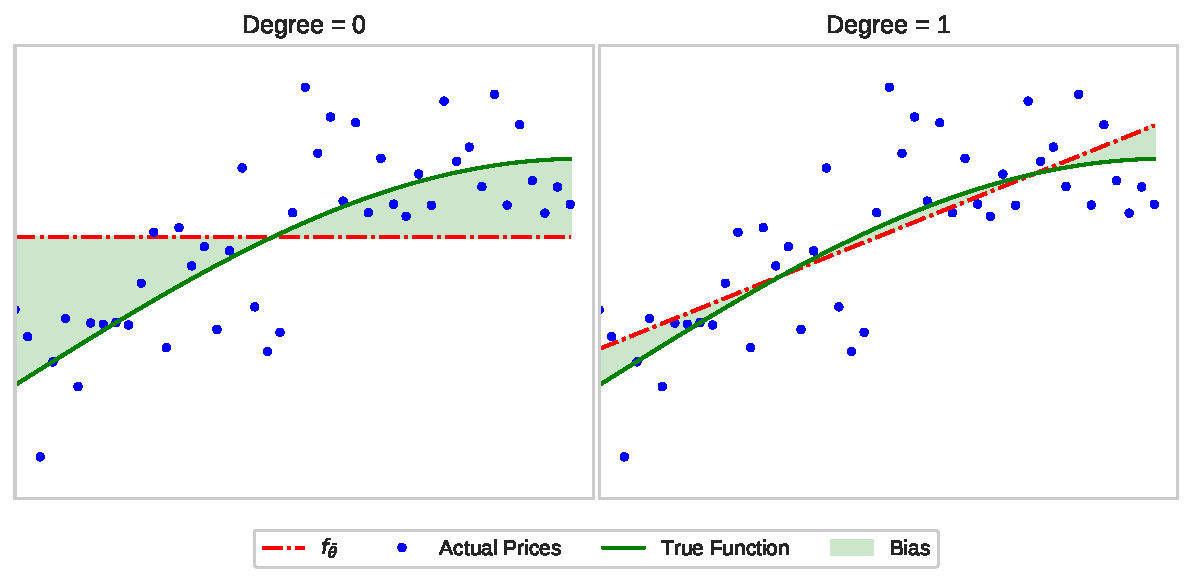
\includegraphics[width=\textwidth]{images/bias7.pdf}
\vspace*{-0.3cm}
\caption{Effect of degree on Bias of the fit}
\end{figure}}
\end{frame}

\begin{frame}{Variance}
\only<1->{Variance of the fit is a measure of how different specific fits can be from each other.}
\only<1->{\begin{figure}
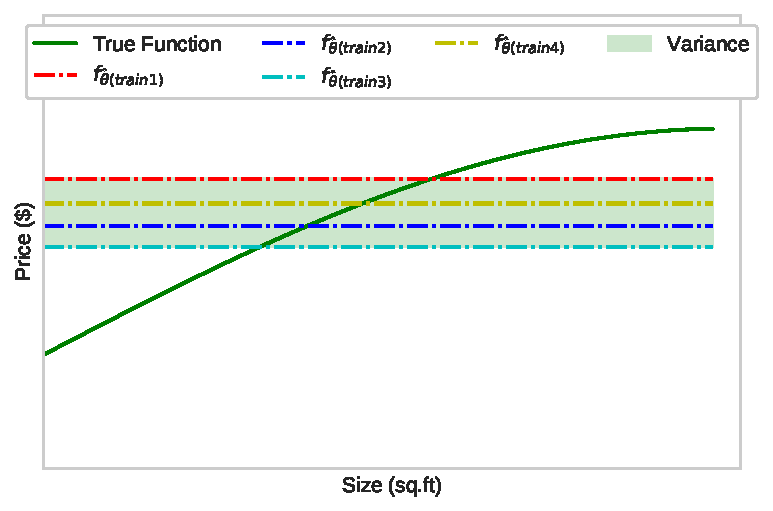
\includegraphics[width=0.7\textwidth]{images/var1.pdf}
\vspace*{-0.3cm}
\caption{Variance of the fit}
\end{figure}}
\end{frame}

\begin{frame}{Variance Contribution}
\only<1>{For Low Complexity \\ $\implies$ variations between curves are less \\ $\implies$ Variance is less}
\only<1>{\begin{figure}
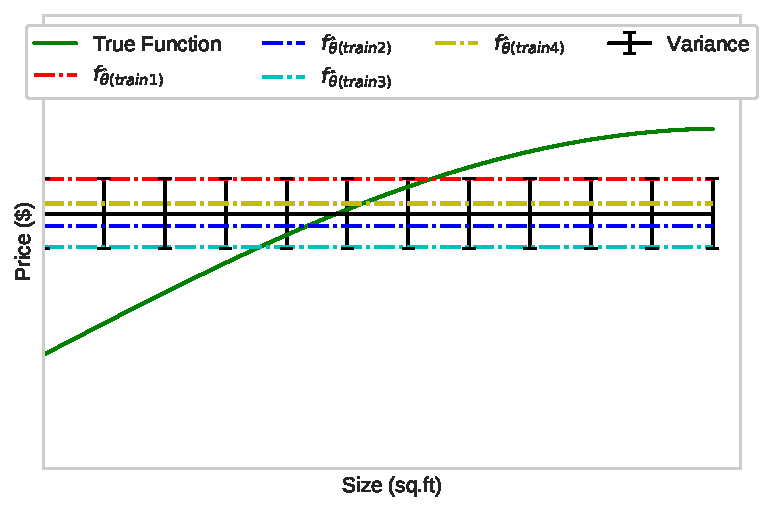
\includegraphics[width=0.7\textwidth]{images/var2.pdf}
\vspace*{-0.3cm}
\caption{Variance of the low complexity fits}
\end{figure}}
\only<2>{\vspace*{0.3cm} For High Complexity we see very high variation}
\only<2>{\begin{figure}
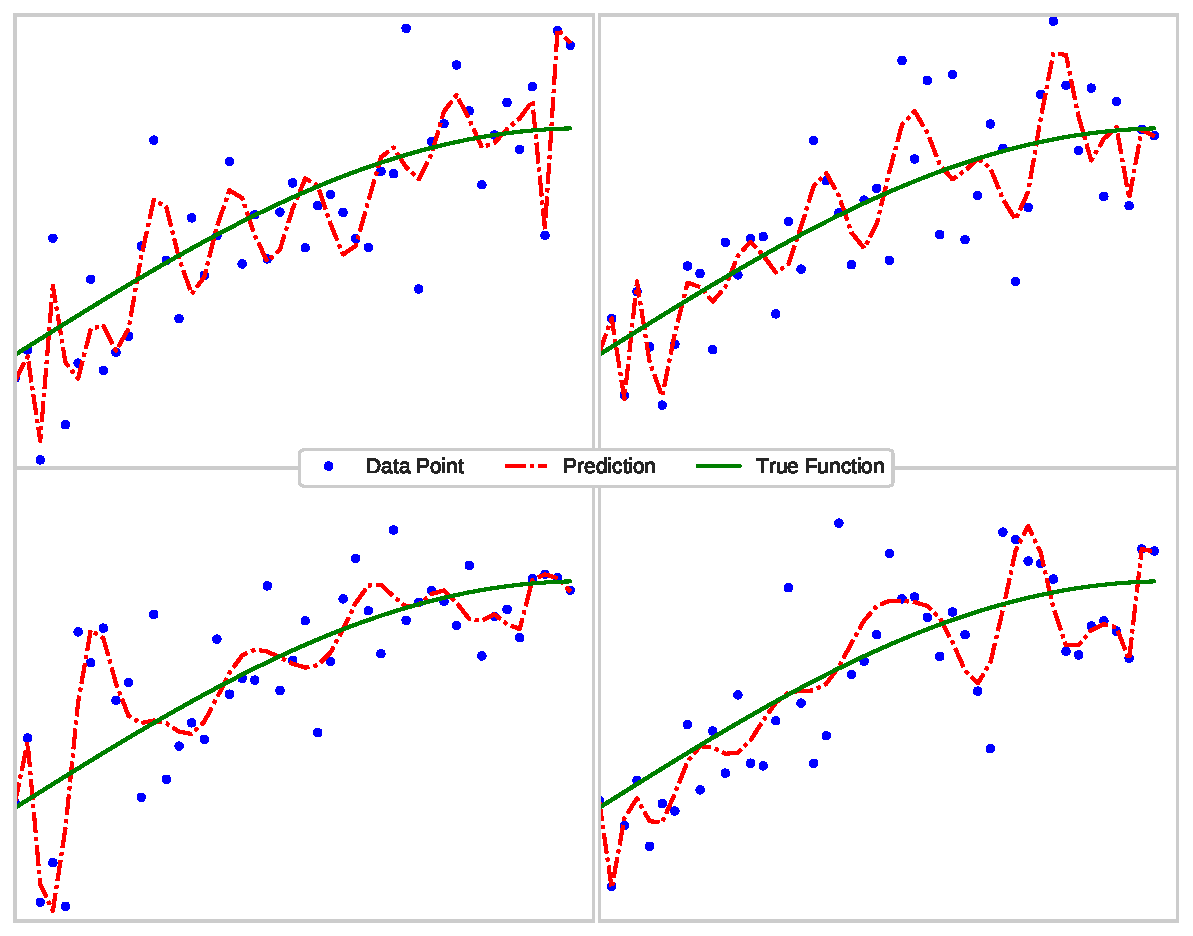
\includegraphics[width=0.7\textwidth]{images/var3.pdf}
\vspace*{-0.3cm}
\caption{Variance in high complexity fits}
\end{figure}}
\only<3>{\vspace*{0.3cm} For High Complexity \\ $\implies$ high variation \\ $\implies$ Variance is high}
\only<3>{\begin{figure}
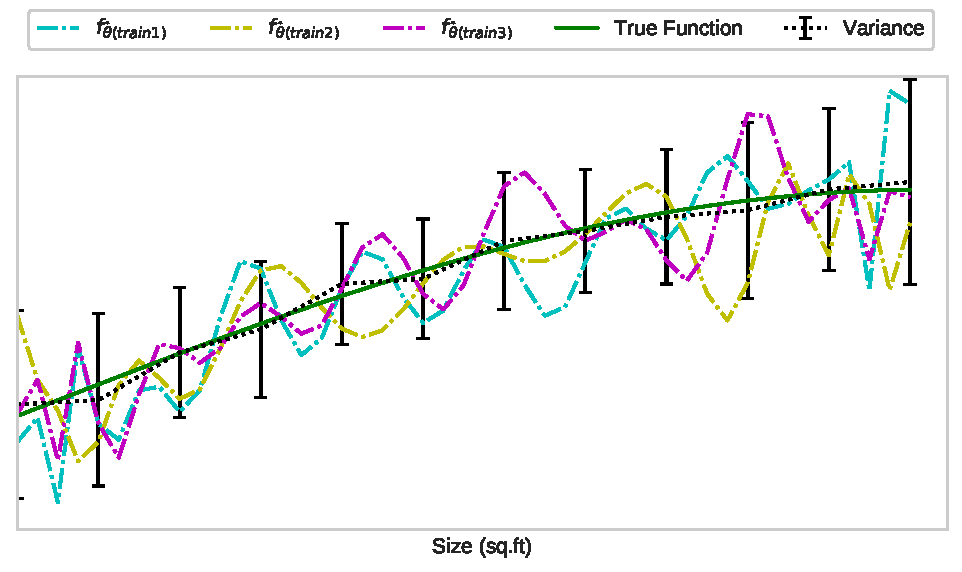
\includegraphics[width=0.8\textwidth]{images/var4.pdf}
\vspace*{-0.3cm}
\caption{Variance of the high complexity fits}
\end{figure}}

\end{frame}

\begin{frame}{The Bias-Variance Trade off}
\textbf{Plot Graph - 3:06 Variance and the bias-variance trade off}
\end{frame}

\section{Mathematically Formulating the Error of a Model}

\begin{frame}{Measuring the goodness of a Model}
To measure the goodness of a model, we have to understand how well it can predict the behavior of the phenomenon.
\pause

This behavior varies due to training set randomness.
\pause 

Therefore, it is important to measure performance \textbf{averaged over all possible training sets} (of size N). 
\pause

$$E_{\text{training set}}[\text{error of } \hat\theta(\text{training set})] $$
gives a measure of the average error by doing an expectation of the errors of all possible training sets of size N.
\end{frame}

\begin{frame}{Expected Prediction Error at a point}
Any prediction made is effected by 3 sources of error:
\begin{itemize}
\item Noise
\item Bias
\item Variance
\end{itemize}
\pause

Therefore, $E_{train} = f(\text{noise, bias, variance}) $

\end{frame}

\begin{frame}{Effect of Noise on the Model}
Noise in a model can be understood \textbf{continue from 5:47 in Formally defining 3 sources of error}
\end{frame}

\begin{frame}{Deriving Expected Prediction Error}
Expected prediction error at $x_t$ = $E_{train,y_t}[(y_t - f_{\hat\theta(train)}(x_t))^2]$\\
\vspace{0.5cm}
\only<2>{
=  $E_{train,y_t}[(          (y_t - f_{\theta(true)}(x_t))     + (f_{\theta(true)}(x_t) -  f_{\hat\theta(train)}(x_t) )            )^2]$
}
\only<3->{
=  $E_{train,y_t}[(      \underbrace{(y_t - f_{\theta(true)}(x_t))}_\text{a}   +   \underbrace{(f_{\theta(true)}(x_t) -  f_{\hat\theta(train)}(x_t) ) }_\text{b}          )^2]$\\
\vspace{0.5cm}
}
\only<4->{
=  $E_{train,y_t}[(a + b) ^ 2]$\\
\vspace{0.5cm}
}
\only<5->{
=  $E_{train,y_t}[a^2 + 2ab + b^2]$\\
\vspace{0.5cm}
}
\only<6->{
(Using Linearity of Expectation)\\
=  $E_{train,y_t}[a^2] + 2E_{train,y_t}[ab] + E_{train,y_t}[b^2]$.......................(Eqn. 1) \\
}

\end{frame}


\begin{frame}{Deriving Expected Prediction Error}
$E_{train,y_t}[a^2]  = E_{train,y_t}[(y_t - f_{\theta(true)}(x_t))^2] $\\
\vspace{0.5cm}
\only<2>{
 \hspace{1.70cm}(Since there is no dependence on training set)\\
\hspace{1.70cm} $ =  E_{y_t}[(y_t - f_{\theta(true)}(x_t))^2] $\\
 \vspace{0.5cm}
}
\only<3->{
 \hspace{1.70cm}($\because$ there is no dependence on training set)\\
 \vspace{0.3cm}
\hspace{1.70cm} $ =  E_{y_t}[\underbrace{(y_t - f_{\theta(true)}(x_t))^2}_\text{$\epsilon^2$}] $\\
 \vspace{0.5cm}
}
\only<3->{
\hspace{1.70cm} $ =  E_{y_t}[\epsilon^2] $\\
 \vspace{0.5cm}
}
\only<4->{
\hspace{1.70cm} $ =  \sigma^2 $(By definition) \\
 \vspace{0.5cm}
}

\only<5->{
$ E_{train,y_t}[a^2] =  \sigma^2  $.................(Eqn. 2)\\
 \vspace{0.5cm}
}
\end{frame}


\begin{frame}{Deriving Expected Prediction Error}
\only<1>{
$E_{train,y_t}[ab]  = E_{train,y_t}[(y_t - f_{\theta(true)}(x_t))(f_{\theta(true)}(x_t) -  f_{\hat\theta(train)}(x_t) )] $\\
\vspace{0.5cm}
}
\only<2->{
$E_{train,y_t}[ab]  = E_{train,y_t}[\underbrace{(y_t - f_{\theta(true)}(x_t))}_\text{$\epsilon$}(f_{\theta(true)}(x_t) -  f_{\hat\theta(train)}(x_t) )] $\\
\vspace{0.5cm}
}
\only<3->{
\hspace{1.70cm} $= E_{train,y_t}[\epsilon (f_{\theta(true)}(x_t) -  f_{\hat\theta(train)}(x_t) )] $\\
\vspace{0.5cm}
}
\only<4>{
\hspace{1.70cm} ( $\because \epsilon$ and $(f_{\theta(true)}(x_t) -  f_{\hat\theta(train)}(x_t))$ are independent)\\
\vspace{0.3cm}
\hspace{1.70cm} $= E_{train,y_t}[\epsilon] \times E_{train,y_t}[(f_{\theta(true)}(x_t) -  f_{\hat\theta(train)}(x_t) )] $\\
\vspace{0.5cm}
}
\only<5->{
\hspace{1.70cm} ( $\because \epsilon$ and $(f_{\theta(true)}(x_t) -  f_{\hat\theta(train)}(x_t))$ are independent)\\
\vspace{0.3cm}
\hspace{1.70cm} $= \underbrace{E_{train,y_t}[\epsilon]}_\text{ = 0 } \times E_{train,y_t}[(f_{\theta(true)}(x_t) -  f_{\hat\theta(train)}(x_t) )] $\\
\vspace{0.25cm}
\hspace{1.70cm} (By definition $\epsilon$ has mean 0)\\
\vspace{0.5cm}
}
\only<6->{
$E_{train,y_t}[ab] = 0$..............(Eqn. 3)
}


\end{frame}

\begin{frame}{Deriving Expected Prediction Error}
$ E_{train,y_t}[b^2] =  E_{train, y_t}[(f_{\theta(true)}(x_t) -  f_{\hat\theta(train)}(x_t) )^2]$\\
\vspace{0.5cm}
\only<2->{
($f_{\theta(true)}(x_t) -  f_{\hat\theta(train)}(x_t)$ is independent of $y_t$)\\
\vspace{0.5cm}
\hspace{1.70cm} $=  E_{train}[(f_{\theta(true)}(x_t) -  f_{\hat\theta(train)}(x_t) )^2]$\\
\vspace{0.5cm}
}
\only<3->{
\hspace{1.70cm} $ = MSE( f_{\hat\theta(train)}(x_t))$\\
\vspace{0.5cm}
}
\only<4->{
$ E_{train,y_t}[b^2] = MSE( f_{\hat\theta(train)}(x_t))$ ............ (Eqn. 4)
}
\end{frame}

\begin{frame}{Deriving Expected Prediction Error}
From Eqn. 1, 2, 3 and 4, we get, \\
\vspace{1cm}
Expected prediction error at $x_t$ = $\sigma^2 + MSE( f_{\hat\theta(train)}(x_t)) $ \\
\vspace{1cm}
Now, we will further simplify the MSE term into bias and variance.
\end{frame}

\begin{frame}{Deriving Expected Prediction Error}
$MSE( f_{\hat\theta(train)}(x_t)) =  E_{train}[(f_{\theta(true)}(x_t) -  f_{\hat\theta(train)}(x_t) )^2]$\\
\vspace{0.5cm}
\only<2>{
$= E_{train}[(   (f_{\theta(true)}(x_t)  -  f_{\hat\theta(avg)}(x_t) ) + (f_{\hat\theta(avg)}(x_t)  -  f_{\hat\theta(train)}(x_t)      ) )^2]$\\
}
\only<3->{
$= E_{train}[(   \underbrace{(f_{\theta(true)}(x_t)  -  f_{\hat\theta(avg)}(x_t) )}_\text{$\alpha$} + \underbrace{(f_{\hat\theta(avg)}(x_t)  -  f_{\hat\theta(train)}(x_t)      )}_\text{$\beta$} )^2]$\\
\vspace{0.5cm}
}
\only<4->{
$= E_{train}[( \alpha + \beta )^2]$\\
\vspace{0.5cm}
}
\only<5->{
$= E_{train}[ \alpha^2 + 2\alpha\beta + \beta ^2]$\\
\vspace{0.5cm}
}
\only<6->{
(Using Linearity of Expectation)
$= E_{train}[ \alpha^2] + 2E_{train}[ \alpha\beta] + E_{train}[ \beta^2]$ ..........(Eqn. 5)\\
\vspace{0.5cm}
}
\end{frame}


\begin{frame}{Deriving Expected Prediction Error}
$E_{train}[\alpha^2]  = E_{train}[(f_{\theta(true)}(x_t)  -  f_{\hat\theta(avg)}(x_t))^2]$\\
\vspace{0.5cm}
\only<2->{
\hspace{1.45cm} $ = E_{train}[bias(f_{\hat\theta}(x_t))^2]$\hfill(By definition of bias)\\
\vspace{0.5cm}
}
\only<3->{
\hspace{1.45cm} $ = bias(f_{\hat\theta}(x_t))^2 $\\
\vspace{0.5cm}
\hspace{1.45cm} ($\because$ bias is not a function of training data)\\

}
\only<4->{
\vspace{0.5cm}
$E_{train}[\alpha^2]  = bias(f_{\hat\theta}(x_t))^2$ .............(Eqn. 6)
}
\end{frame}


\begin{frame}{Deriving Expected Prediction Error}
$E_{train}[\alpha\beta] $ \\
$= E_{train}[(f_{\theta(true)}(x_t)  -  f_{\hat\theta(avg)}(x_t))(f_{\hat\theta(avg)}(x_t)  -  f_{\hat\theta(train)}(x_t)   )]$\\
\vspace{0.5cm}
\only<2->{
$ = E_{train}[bias \times (f_{\hat\theta(avg)}(x_t)  -  f_{\hat\theta(train)}(x_t)   )]$\\
\vspace{0.5cm}
}
\only<3->{
$ = bias \times E_{train}[f_{\hat\theta(avg)}(x_t)  -  f_{\hat\theta(train)}(x_t)  ]$\\
\vspace{0.5cm}
($\because$ bias is not a function of training data)\\
\vspace{0.5cm}
}
\only<4->{
$ = bias \times \left( E_{train}[f_{\hat\theta(avg)}(x_t)]  -  E_{train}[f_{\hat\theta(train)}(x_t) ] \right)$\\
\vspace{0.5cm}
}
\only<5>{
$ = bias \times \left( f_{\hat\theta(avg)}(x_t)  -  f_{\hat\theta(avg)}(x_t)  \right) $\\
\vspace{0.5cm}
($\because f_{\hat\theta(avg)}(x_t) =  E_{train}[f_{\hat\theta(train)}(x_t)$ )\\
\vspace{0.5cm}
}
\only<6->{
$ = bias \times \left( f_{\hat\theta(avg)}(x_t)  -  f_{\hat\theta(avg)}(x_t)  \right) $\\
\vspace{0.5cm}
$E_{train}[\alpha\beta]  = 0$..........................(Eqn. 7) 
\vspace{0.5cm}
}

\end{frame}



\begin{frame}{Deriving Expected Prediction Error}
$E_{train}[\beta^2]  = E_{train}[(f_{\hat\theta(avg)}(x_t)  -  f_{\hat\theta(train)}(x_t) )^2]$ \\
\vspace{0.5cm}
\only<2->{
\hspace{1.45cm} $=  E_{train}[(f_{\hat\theta(train)}(x_t) - f_{\hat\theta(avg)}(x_t))^2]$\\
\vspace{0.5cm}
}
\only<3->{
\hspace{1.45cm} $=  E_{train}[(f_{\hat\theta(train)}(x_t) - E_{train}[(f_{\hat\theta(train)}(x_t)])^2]$\\
\vspace{0.5cm}
\hspace{1.45cm} ($\because f_{\hat\theta(avg)}(x_t) = E_{train}[(f_{\hat\theta(train)}(x_t)] $ )\\
\vspace{0.5cm}
}
\only<4->{
\hspace{1.45cm} $= variance(f_{\hat\theta}(x_t))$\\
\vspace{0.5cm}
}
\only<5->{
$E_{train}[\beta^2] = variance(f_{\hat\theta}(x_t))$...............(Eqn. 8)\\
}

\end{frame}



\begin{frame}{Deriving Expected Prediction Error}
From Eqn. 1 - 8, we get, \\
\vspace{0.5cm}
Expected prediction error at $x_t$ \\
\vspace{0.5cm}
$ = \sigma^2 + MSE( f_{\hat\theta(train)}(x_t)) $\\
\vspace{0.5cm}
$ = \sigma^2 +bias(f_{\hat\theta}(x_t))^2 + variance(f_{\hat\theta}(x_t))$

\end{frame}





\end{document}